The preceding chapter established that the self-shielding correction factor $C_T$ can be computed by Monte Carlo sampling of SLBW resonances from average parameters, and that this computation must be embedded within a fitting loop to determine those parameters from experimental data. This chapter describes the implementation of that procedure within SAMMY, including the physics models, sampling algorithms, and code validation required to produce self-shielded theoretical observables from URR parameters.

Previously, evaluating URR data was a tedious, manual cycle, requiring the evaluator to iterate between SAMMY and SESH. The process required the evaluator to convert a transmission measurement $\langle T \rangle$ to a non-physical ``uncorrected'' cross section:
\begin{equation}
    \overline{\sigma} = -\frac{1}{n} \ln{ \langle T \rangle}
\end{equation}
where $n$ is the atomic thickness of the sample in atoms/barn. As discussed in the introduction, this derived quantity is not the true average cross section but rather a self-shielded cross section that depends on experimental conditions (sample thickness, temperature, composition, etc.) and needed to be corrected before fitting with SAMMY.
This was converted into the \textit{true} average cross section by use of the correction factor calculated from SESH, which was then fit with SAMMY.

Once new parameters were obtained, they were used to calculate a new correction factor. This was then used to obtain a new `corrected' cross section, and a new fit was performed, producing new resonance parameters. This process was repeated until the resonance parameters converged onto a final value.

The implementation described in the following sections integrates the self-shielding correction capabilities of SESH directly into SAMMY’s fitting engine. This creates a new, streamlined workflow where the evaluator provides the actual measurement data—such as average transmission or capture yield—directly to the code. SAMMY now internally calculates the necessary self-shielding correction factors during each iteration, directly comparing the theoretical values to the experimental observable. The new and improved workflow is shown in \autoref{fig:current-workflow}.
\begin{figure}[h]
    \centering
    \includegraphics[width=1\linewidth]{Implementation/Figures/ImprovedWorkflow.pdf}
    \caption{Current SAMMY workflow for processing self-shielded URR data}
    \label{fig:current-workflow}
\end{figure}

While the code SESH was used to provide a blueprint for performing self-shielding corrections, its implementation into SAMMY required a near-total rewrite of the original code. This overhaul was required in order to modernize SESH's interface such that it integrated cleanly into SAMMY, resolve bugs that had been propagated through SESH's development history, and improve the physics models such that:
\begin{enumerate}
    \item Approximations which significantly impacted results were removed
    \item SESH and SAMMY utilize the same underlying physics models, ensuring consistency throughout the code.
\end{enumerate}

The following sections will discuss software refactoring (bug fixes, improved physics models) required to perform the self-shielding corrections in order to accomplish these goals. The specific theoretical measurement validation will be discussed in their respective chapters, as will the fitting procedure.

\section{URR Representation in SAMMY}
\label{sec:urr-in-sammy}

The average cross section in the URR is typically described using the Hauser-Feshbach statistical theory\cite{Hauser1952}\cite{Moldauer1963}, which provides a framework for nuclear reactions proceeding through a compound nucleus when many overlapping resonances are present and individual resonance effects are averaged out. The energy-averaged total cross section for an incoming channel $c$, defined by its orbital angular momentum $\ell$ and total angular momentum $J$, can be expressed as\cite{jeff18}:

\begin{equation}
    \label{eq:hauser-feshbach-cross-section}
    \langle \sigma_c \rangle =
    \frac{2 \pi g_c}{k_c^2} \left\{
    1 - \frac{
            \cos{ ( 2 \phi_c)} \left[
                1 - \pi^2P_c^2 s_c^2 -  \left( P_c R_c^\infty \right)^2
            \right]
            + \sin{(2 \phi_c)} 2 P_c R_c^\infty
        }{
            \left( 1 + \pi P_c s_c \right)^2 + \left( P_c R_c^\infty \right)^2
    }
    \right\}
\end{equation}
where $k_c$, $g_c$, and $\phi_c$ are the neutron wave number, statistical spin factor, and hard-sphere scattering phase shift as defined in \autoref{sec:slbw-for-sampling}. The quantities specific to the Hauser-Feshbach formulation are:
\begin{itemize}
    \item $P_c$ is the neutron penetrability for channel $c$, a function of $\ell$ and the dimensionless channel radius parameter $\rho_c = k_c a_c$, where $a_c$ is the channel radius,
    \item $R_c^\infty$ is the distant-level parameter, which accounts for the cumulative effect of all resonances outside the energy range of interest on the average cross section\cite{Lynn1968},
    \item $s_c$ is the pole strength, related to the strength function $\widetilde{S}_c$ by $s_c = \widetilde{S}_c a_c \sqrt{E}/(2 k_c)$. The strength function characterizes the average reduced neutron width per unit energy interval for a given orbital angular momentum $\ell$\cite{atlas}.
\end{itemize}

The parameters that distinguish this average cross section from a simple energy average of resolved resonance region cross sections are the distant-level parameter $R^\infty_c$ and the strength function $\widetilde{S}_c$. Together with the s-wave average level spacing $D_0$, these constitute the set of URR parameters that SAMMY uses to describe the average cross section. These are defined on an $\ell$-basis (i.e., $S_\ell$, $R_\ell^\infty$) and are the parameters that are either input by the evaluator or varied during the fitting process.


\section{Converting Optical Model Parameters to Statistical Resonance Parameters}
\label{sec:param-conversion}
    As described in \autoref{sec:mc-sampling-from-average-parameters}, accurately modeling resonance self-shielding requires stochastically sampling resonance ladders to account for cross-section variance. While \autoref{eq:hauser-feshbach-cross-section} provides a convenient analytical form for the \textit{average} cross section, it does not capture the fluctuations around that average. Computing self-shielding correction factors therefore requires generating statistical realizations of the cross section from Monte Carlo--sampled resonance ladders, as described in the theory chapter.

    This presents a fundamental mismatch between two representations of URR nuclear data. The Hauser-Feshbach average cross section (\autoref{eq:hauser-feshbach-cross-section}) is parameterized by optical-model quantities---the strength function $S_\ell$, the distant-level parameter $R_\ell^\infty$, and the s-wave average level spacing $D_0$---all defined on an orbital angular momentum ($\ell$) basis. These $\ell$-dependent parameters are natural for describing the average cross section and are the quantities that SAMMY varies during the fitting process.

    However, the Monte Carlo resonance simulation described in \autoref{sec:sampling-parameters} requires a different set of parameters: the $J$-dependent average level spacing $D_J$ and the channel-dependent average neutron width $\langle \Gamma_{n,J}^{\ell} \rangle$. Actual nuclear resonances are associated with specific compound nuclear states, each characterized by a total angular momentum $J$, orbital angular momentum $\ell$, and parity $\pi$\cite{Lynn1968}. The $\ell$-dependent optical-model parameters cannot be used to generate resonance ladders directly; they must first be converted to channel-dependent statistical resonance parameters.

    This conversion can be summarized as three steps:
    \begin{enumerate}
        \item Convert $D_0$ to $D_J$: determine the $J$-dependent level spacing from the s-wave level spacing using a nuclear level density model.
        \item Convert $S_\ell, D_J$ to $\langle \Gamma_{n,J}^{\ell} \rangle$: calculate the average neutron width for each channel from the strength function, level spacing, and penetrability.
        \item Convert $R_\ell^\infty$ to $R'_\ell$: determine the effective scattering radius from the distant-level parameter for use in calculating the hard-sphere phase shift in the SLBW equation.
    \end{enumerate}
    The following sections describe each of these conversions. Once complete, the channel-dependent parameters ($D_J$, $\langle \Gamma_{n,J}^{\ell} \rangle$, and the phase shifts via $R'_\ell$) are used to generate sampled resonance ladders and compute cross-section realizations via the SLBW equations described in \autoref{sec:slbw-for-sampling}.


    \subsection{Calculating Available Channels}
        \label{ssec:channels}
    
        For an isotope with a ground-state spin $I$ interacting with a neutron (which has an intrinsic spin of $s_n = 1/2$), there are two possible channel spins\cite{Blatt1952}: $s_{-} = I - 1/2$ and $s_{+} = I + 1/2$. For a given orbital angular momentum $\ell$, this leads to two separate sets of allowed total angular momentum $J$ values, one for each channel spin:
        \begin{align}
            \mathbf{J}_{-} &= \left\{ \left|s_{-} - \ell\right|, \left|s_{-} - \ell\right| + 1, \cdots, s_{-} + \ell \right\}\\
            \mathbf{J}_{+} &= \left\{ \left|s_{+} - \ell\right|, \left|s_{+} - \ell\right| + 1, \cdots, s_{+} + \ell \right\}
        \end{align}
        A common assumption in URR evaluations is that average resonance parameters are independent of parity\cite{endf-manual}, i.e., the statistical properties of resonances with quantum numbers $(J, \ell, \pi = (-1)^\ell)$ are treated as identical to those with $(J, \ell+1, \pi = (-1)^{\ell+1})$ when both have the same $J$. As a consequence, only $J$ and $\ell$ need to be considered when generating resonance ladders. Instead, the important factor to track is the multiplicity $\mu$: if the same $J$ value can be formed from both $s_{+}$ and $s_{-}$ channel spins, then $\mu = 2$; otherwise $\mu = 1$. This overlap is illustrated in \autoref{eq:multiplicities}:

        \begin{equation}
            \label{eq:multiplicities}
            \begin{array}{rrrrrrrr}
            \mathbf{J}_{-}: & \{ & \left|s_{-} - \ell\right|, & \left|s_{-} - \ell\right| + 1, & \dots, & s_{-} + \ell ~ & & \} \\
            \mathbf{J}_{+}: & \{ & & \left|s_{+} - \ell\right|, & \dots, & s_{+} + \ell-1, & s_{+} + \ell & \} \\[1em] \hline \\[-0.5em]
            \mathbf{J}_{tot}: & \{ & \left|s_{-} - \ell\right|, & \left|s_{+} - \ell\right|, & \dots, & s_{-} + \ell, & s_{+} + \ell & \} \\
            \mathbf{\mu}_J: & \{ & 1, & 2, & \dots, & 2, & 1 & \} \\
            \end{array}
        \end{equation}
        The physical significance of the multiplicity is that it determines the number of degrees of freedom for the $\chi^2$ distribution from which neutron widths are sampled\cite{PorterThomas1956}. When $\mu = 2$, the neutron width is sampled from a $\chi^2$ distribution with two degrees of freedom rather than one. By utilizing this assumption, the number of resonance ladders that must be independently sampled is nearly halved, since two channel spins sharing the same $J$ are treated as a single effective channel.
    
        The complete vector of unique channels, $\mathbf{C}$, is constructed by compiling the $\mathbf{J}_{tot}$ and $\boldsymbol{\mu}_J$ vectors for each orbital angular momentum $\ell$ up to the maximum $\ell$ value included in the evaluation. Each element of $\mathbf{C}$ is defined as:
        \begin{equation}
        \label{eq:channel-list}
            c_i = (J_i, \ell_i, \mu_i)
        \end{equation}
        which describes the complete set of quantum states available for resonance simulation for a given nuclide.

    \subsection{Calculating $J$-Dependent Level Spacings}
        \label{ssec:level-density}
        With the set of available channels established, the next step is determining the average level spacing $D$ for each channel. This calculation is simplified by two key observations. The first is that the average level spacing is empirically observed to be independent of $\ell$\cite{level-spacing-statistics}\cite{Lynn1968}. The second is the assumption established in \autoref{ssec:channels} that average channel parameters are independent of parity $\pi$. Consequently, the average level spacing depends only on $J$:
        \begin{equation}
            D_{\ell,J,\pi} = D_J
        \end{equation}
        and only the $J$ dependence needs to be accounted for when calculating channel-by-channel level spacings from the input s-wave level spacing $D_0$.
        
        A significant update was implemented in the methodology for determining the $J$-dependent level spacing $D_J$. The original SESH code calculated this value using a simple relation involving the statistical spin factor $g_J$:
        \begin{equation}
            \label{eq:simple-j-dependency}
            D_J = \frac{D_0}{g_J}
        \end{equation}
        This approximation assumes that the level density is proportional to $g_J = (2J+1)/[2(2I+1)]$, which is only valid when the spin cutoff parameter is large relative to $J$. The primary motivation for updating this formula was to enable a more physically realistic model that properly accounts for the energy and $J$ dependence of level spacings.
        
        The updated methodology uses the Bethe level density formula\cite{Bethe1936}\cite{gc-leveldensity} to describe the relationship between $D_0$ and $D_J$:
        \begin{equation}
            \label{eq:bethe-formula}
            \frac{1}{D_J} = \frac{1}{D_0}
            \left\{ \exp{ \left[ \frac{-J^2}{2\sigma_J^2(E)}\right]} - \exp{ \left[ \frac{-(J+1)^2}{2\sigma_J^2(E)}\right]}
            \right\} 
        \end{equation}
        where $\sigma_J^2$ is the spin cutoff parameter (not to be confused with cross section $\sigma$), which characterizes the width of the angular momentum distribution of nuclear levels. The spin cutoff parameter is described by\cite{gc-leveldensity}:
        \begin{equation}
            \sigma_J^2(E) = 0.14592 \cdot (A+1)^{2/3}\sqrt{a_{\text{ld}}(E + B_E - P_E)}
        \end{equation}
        in which $A$ is the mass number of the target nucleus, $a_{\text{ld}}$ is the level density parameter (in MeV$^{-1}$), $B_E$ is the back-shift energy (in MeV), and $P_E$ is the pairing energy (in MeV). These quantities are obtained from the Gilbert-Cameron composite level density model\cite{gc-leveldensity}. The Bethe formula allows $D_J/D_0$ to evolve as a function of energy more realistically compared to the simple approximation in \autoref{eq:simple-j-dependency}, particularly for high-$J$ states and at higher energies where the spin cutoff parameter varies significantly.
        
        The energy dependence of $D_0$ itself is also accounted for using the Gilbert-Cameron level density model\cite{gc-leveldensity}. This aspect already matched SAMMY's existing implementation and was therefore left unchanged.

        The validation of this model was done by comparing the new calculated level densities with the new \textsuperscript{181}Ta evaluation from ENDF-8.1\cite{endf-8.1}.

        \begin{figure}[H]
            \centering
            \begin{adjustbox}{width=1.2\textwidth, center}
            \includegraphics{Implementation/Figures/validating-level-spacing.pdf} 
            \end{adjustbox}
            \caption{Validating the improved level spacing model in SESH with \textsuperscript{181}Ta spin groups from ENDF-8.1 Evaluation}
            \label{fig:level=spacing=validation}
        \end{figure}

        As shown in \autoref{fig:level=spacing=validation}, the results from the improved level density formula now correctly match the $^{181}$Ta evaluation. While the simpler model in \autoref{eq:simple-j-dependency} approximates the level spacing adequately for s-wave channels, the two formulas diverge at higher $\ell$ values where the spin cutoff parameter plays a larger role. Implementing the Bethe formula (\autoref{eq:bethe-formula}) resolves these approximations.

    \subsection{Converting Strength Functions to Average Neutron Widths}
    \label{ssec:neutron-widths}
        With the complete set of available channels and the $J$- and $E$-dependent level spacings calculated in the previous sections, the per-channel average neutron width $\langle \Gamma_{n,J}^{\ell} \rangle$ can be calculated. This is the quantity required by the Porter-Thomas sampling described in \autoref{sec:sampling-parameters}. For each unique channel $(\ell, J)$, it is given by\cite{Lynn1968}\cite{atlas}:
        \begin{equation}
            \label{eq:avg-neut-width}
            \langle \Gamma_{n,J}^{\ell} \rangle = \mu_{\ell,J}\, D_J\, S_\ell\, V_{\ell}(E)\, \sqrt{E}
        \end{equation}
        where:
        \begin{itemize}
            \item $\mu_{\ell,J}$ is the multiplicity of the $(\ell, J)$ channel (as defined in \autoref{ssec:channels}),
            \item $D_J$ is the $J$-dependent average level spacing (from \autoref{eq:bethe-formula}),
            \item $S_\ell$ is the strength function for orbital angular momentum $\ell$ (either input or fit to experimental data),
            \item $V_{\ell}(E)$ is the neutron penetrability factor\cite{Blatt1952}, which accounts for the energy dependence of the neutron width and depends on $\ell$ and the dimensionless parameter $\rho = k_c a_c$,
            \item $E$ is the incident neutron energy.
        \end{itemize}
        The penetrability factor $V_\ell$ has the following $\ell$-dependent forms:
        \begin{equation}
        \label{eq:penetration-factor}
            V_\ell = \begin{cases}
                \quad\quad\:\:\:\displaystyle\rho & \ell=0,\\[12pt]
                \quad\:\:\displaystyle\frac{\rho^3}{1 + \rho^2} & \ell=1,\\[12pt]
                \displaystyle\frac{\rho^5}{9 + 3\rho^2 + \rho^4} & \ell=2
                %&\displaystyle\frac{\rho^7}{225 + 45\rho^2 + 6\rho^4 + \rho^6} & \ell=3
            \end{cases}
        \end{equation}

        The parameter $\rho$ is the dimensionless channel radius parameter, defined as
        \begin{equation}
            \rho = k_c\, a_c
            \label{eq:channel-radius-param}
        \end{equation}
        in which $a_c$ is the channel radius and $k_c$ is the neutron wave number.

        Note that the penetrability $V_\ell$ appearing in \autoref{eq:avg-neut-width} is the same quantity that enters the SLBW formulation of \autoref{sec:slbw-for-sampling} through the energy dependence of the neutron width. Putting all of these pieces together, the average neutron width is calculated from the input $\ell$-dependent parameters and can be used to generate Monte Carlo samples of individual neutron widths via the Porter-Thomas distribution as described in \autoref{sec:sampling-parameters}.
        
    \subsection{Converting Inelastic Strength to Inelastic Widths}
        \label{ssec:inelastic-strength}
        The original SESH code determined the inelastic neutron width using a form identical to \autoref{eq:avg-neut-width}, treating the inelastic channel as if it were elastic with a simple average width. This approach is a poor physical approximation, as it fails to account for the discrete nature of nuclear excited states that serve as outgoing channels for inelastic scattering.

        The ENDF-6 format manual\cite{endf-manual} provides guidance for calculating the inelastic width by summing over all energetically accessible excited states and all allowed outgoing orbital angular momenta. The improved implementation calculates the inelastic width as:
        \begin{equation}
            \label{eq:inelastic-width}
            \langle \Gamma_{n',J}^\ell \rangle = \sum_{i,\ell'} \mu_{J,\ell'}\, D_J\, S_{\ell'}\, V_{\ell'}(E - E_i)\, \sqrt{E - E_i}
        \end{equation}
        Here, the sum is over all excited states $i$ with excitation energy $E_i < E$ (i.e., only energetically accessible states) and all possible outgoing orbital angular momenta $\ell'$ consistent with angular momentum and parity conservation. The penetrability $V_{\ell'}$ and $\sqrt{E-E_i}$ are evaluated at the outgoing neutron energy $(E - E_i)$. This more realistically accounts for the inelastic neutron width than the original SESH formula, and is consistent with SAMMY's calculated inelastic widths.

    \subsection{Calculating Potential Scattering}
        \label{ssec:pot-scat}

        The final component required for the cross-section simulation is the potential scattering cross section\cite{Teichmann1952}. As shown in the SLBW total cross section (\autoref{eq:slbw}), the $\sin^2\phi_c$ term exists outside the resonance sum and represents the contribution of potential (shape-elastic) scattering. When summed over all channels, the total potential scattering cross section is\cite{t2}:
        \begin{equation}
            \label{eq:potential-scattering}
            \sigma_p = \frac{ 4 \pi}{k^2} \sum_\ell (2\ell +1) \sin^2{\phi_\ell}
        \end{equation}
        where the sum extends over all orbital angular momenta included in the evaluation. The key quantity is $\phi_\ell$, the hard-sphere phase shift, which is calculated as a function of $\ell$ and the dimensionless parameter $\hat{\rho}$:

    \begin{equation}
        \label{eq:phase-shift}
        \phi_\ell = \begin{cases}
            \hat{\rho} & \ell=0,\\[12pt]
            \hat{\rho} - \arctan{\hat{\rho}} & \ell=1,\\[12pt]
            \displaystyle\hat{\rho} - \arctan{\frac{3\hat{\rho}}{3 - \hat{\rho}^2} } & \ell=2\\[12pt]
            %\displaystyle{\hat{\rho} - \arctan{\frac{15\hat{\rho} - \hat{\rho}^3}{15 - 6\hat{\rho}^2} } }  & \text{if}\quad \ell=3\[14pt]
        \end{cases}
    \end{equation}

        The parameter $\hat{\rho}$ is defined analogously to $\rho$ (\autoref{eq:channel-radius-param}), but uses the effective scattering radius $R'_\ell$ in place of the channel radius $a_c$:
        \begin{equation}
            \hat{\rho} = k_c\, R'_\ell
        \end{equation}
        The effective scattering radius $R'_\ell$ connects the distant-level parameter $R^\infty_\ell$ (one of the input parameters to SAMMY) to the phase shift used in the SLBW cross-section calculation.

        In the low-energy limit for s-waves, the effective scattering radius $R'_0$ can be calculated from the channel radius $a_c$ and the distant-level parameter $R_0^\infty$ using the well-known approximation\cite{Lynn1968}:
        \begin{equation}
            R'_0 = a_c (1 - R_0^\infty) \label{eq:rprime-swave}
        \end{equation}
        However, for analyses that extend to higher energies or include higher orbital angular momenta ($\ell > 0$), this s-wave approximation is inadequate\cite{jeff18}\cite{Lynn1968}. A more general model is required to accurately describe the potential scattering contribution to the cross section.
        
        The generalized SPRT (Single Particle Resonance Theory) method\cite{sprt} provides an improved model that extends beyond the s-wave low-energy approximation. It gives an approximate relationship for the effective scattering radius $R'_\ell$ that accounts for higher-order partial waves:
        \begin{equation}
            \label{eq:sprt}
            R_\ell^{\prime} \approx a_c\left[1-(2\ell+1) R_\ell^{\infty}\right]^{1/(2\ell+1)}
        \end{equation}
        For $\ell = 0$, \autoref{eq:sprt} reduces to \autoref{eq:rprime-swave}. For $\ell > 0$, this equation provides a more physically appropriate description of the effective scattering radius, which is important for nuclei where p-wave and d-wave contributions are significant in the URR.

\section{Cross-Section Sampling Procedure}
\label{sec:sampling-procedure}

With all channel-dependent parameters established by the conversions in the preceding sections, the Monte Carlo sampling procedure outlined conceptually in \autoref{sec:sampling-parameters} can now be stated concretely. The goal is to generate an ensemble of cross-section realizations $\{\sigma_1, \sigma_2, \ldots, \sigma_N\}$ from which the correction factor $C_T$ is computed.

For each realization $i$, the following steps are performed for every channel $c_j = (J_j, \ell_j, \mu_j)$ in the channel list (\autoref{eq:channel-list}):

\begin{enumerate}
    \item \textbf{Sample a resonance ladder.} A sequence of resonance energies is generated by sampling level spacings from the Wigner distribution:
    \begin{equation}
        \label{eq:wigner-distribution}
        P(s) = \frac{\pi s}{2 D_J^2} \exp\left(-\frac{\pi s^2}{4 D_J^2}\right)
    \end{equation}
    where $D_J$ is the $J$-dependent average level spacing from \autoref{eq:bethe-formula} and $s$ is the sampled spacing. These spacings are accumulated to produce a resonance ladder:
    \begin{equation}
        E_{r+1} = E_r + s
    \end{equation}
    In practice, SESH does not build a full resonance ladder across the entire URR; instead, it samples only the resonances in the vicinity of the energy of interest using a weighted Wigner distribution, as described in \autoref{sec:weighted-wigner-validation}.

    \item \textbf{Sample neutron widths.} For each resonance $r$ in the ladder, the neutron width is sampled from a $\chi^2$ distribution with $\mu_j$ degrees of freedom, scaled by the average neutron width:
    \begin{equation}
        \label{eq:porter-thomas}
        \Gamma_{n,r} = \langle \Gamma_{n,J}^{\ell} \rangle \cdot \frac{X}{\mu_j}, \quad X \sim \chi^2(\mu_j)
    \end{equation}
    where $\langle \Gamma_{n,J}^{\ell} \rangle$ is computed from the strength function via \autoref{eq:avg-neut-width}. When the multiplicity $\mu_j = 1$, this reduces to the Porter-Thomas distribution\cite{Porter1956}, a $\chi^2$ with one degree of freedom:
    \begin{equation}
        P(x) = \frac{e^{-x/2}}{\sqrt{2\pi x}}
    \end{equation}
    where $x = \Gamma_n / \langle \Gamma_n \rangle$. As discussed in \autoref{sec:sampling-parameters}, this is the dominant source of cross-section variance. The radiation width $\Gamma_\gamma$ and inelastic width $\Gamma_{n'}$ (\autoref{eq:inelastic-width}) are treated as constant for all resonances within a given channel, consistent with their large effective degrees of freedom.

    \item \textbf{Assemble the total width and compute the cross section.} The total width for each resonance is:
    \begin{equation}
        \Gamma_{tot,r} = \Gamma_{n,r} + \Gamma_\gamma + \Gamma_{n'}
    \end{equation}
    The sampled parameters $(E_r, \Gamma_{n,r}, \Gamma_{tot,r})$ are substituted into the SLBW equation (\autoref{eq:slbw}) to compute the cross section for channel $c_j$. The Doppler-broadened line shapes $\psi$ and $\chi$ are evaluated at the sample temperature using the Faddeeva function (\autoref{eq:faddeeva}).
\end{enumerate}

The total cross section for realization $i$ is obtained by summing over all channels:
\begin{equation}
    \sigma_i = \sum_j \sigma_{c_j}
\end{equation}
Partial cross sections (e.g., capture, \autoref{eq:slbw-capture}) are computed simultaneously from the same sampled resonance parameters. This procedure is repeated $N$ times to produce the ensemble $\{\sigma_1, \sigma_2, \ldots, \sigma_N\}$. From this ensemble, the mean cross section $\langle\sigma\rangle$ and the average transmission $\langle T \rangle = \frac{1}{N}\sum_i e^{-n\sigma_i}$ are computed, yielding the correction factor $C_T$ as defined in \autoref{eq:ct-sesh-form}.

The following sections validate individual components of this procedure: the weighted Wigner sampling scheme (\autoref{sec:weighted-wigner-validation}), the Doppler broadening implementation, and the overall cross-section distribution (\autoref{sec:cross-section-validation}).

\section{Validation of the Weighted Wigner Distribution}
\label{sec:weighted-wigner-validation}
As described in the preceding section, generating a statistical resonance ladder involves sequentially sampling level spacings $s$ from the Wigner distribution (\autoref{eq:wigner-distribution}). However, building whole ladders would be extremely inefficient for SESH's purposes. While NJOY and FRENDY need to sample across the entire URR, SESH is designed to correct at specific energies.

To circumvent this inefficiency, only the resonances directly around the energy of interest are sampled. The issue with doing this is that a neutron is proportionally more likely to fall into a wider level spacing than a narrow one, assuming that neutrons are distributed uniformly across all observed resonances. To address this, Fr\"{o}hner\cite{jeff18} developed a weighted sampling scheme to sample level spacings weighted by their size, which can be represented as:
\begin{equation}
    \label{eq:weighted-wigner}
    P_{weighted}(s) = \frac{s \cdot P(s)}{\displaystyle\int_0^\infty s' \cdot P(s') ds'}
\end{equation}

In order to validate Fr\"{o}hner's implementation of \autoref{eq:weighted-wigner}, a sequence of $10^7$ resonances was built,
\begin{equation}
    \left\{\lambda_0, \lambda_1, \lambda_2, \dots, \lambda_{N-1}, \lambda_{N} \right\}
\end{equation}
in which
\begin{equation}
    \lambda_{r+1} = \lambda_r + s_r
\end{equation}
where $s_r$ was sampled from \autoref{eq:wigner-distribution}. A random energy $E_{rand}$ was randomly sampled from a uniform distribution over the range $[
\lambda_0,\lambda_N]$, and identified a resonance $i$ which fit the criteria:
\begin{equation}
    \lambda_i \leq E_{rand} < \lambda_{i+1}
\end{equation}
Therefore, the sampled $s_{observed}$ was determined by:
\begin{equation}
    s_{observed} = \lambda_{i+1} - \lambda_{i}
\end{equation}
This observed width was collected into a set and compared to the sampled values from Fr\"{o}hner's implementation of \autoref{eq:weighted-wigner}.
\begin{figure}[H]
    \centering
    \includegraphics[width=0.75\linewidth]{Implementation/Figures/weighted-wigner-validation.pdf}
    \caption{Validation of Fr\"{o}hner's implementation of the weighted Wigner level spacing algorithm}
    \label{fig:weighted-wigner}
\end{figure}

As shown in \autoref{fig:weighted-wigner} Fr\"{o}hner's implementation of the weighted Wigner distribution successfully replicates the distribution of observed widths when weighting according to energy, and can be used to accelerate the sampling routine without a loss of accuracy.

\section{Doppler Broadening}

When testing SESH theoretical values, there was an observed disagreement in cross-section variance at higher energies for capture cross sections.
    The primary cause of the disagreement was determined to be the result of an error in the Doppler broadening subroutine that was originally present in SESH. In order to perform the Doppler broadening, the Faddeeva function (as defined in \autoref{eq:faddeeva}) is utilized. The issue was in the original algorithm, in cases where $\beta$ was less than 0.01. Recall from \autoref{eq:doppler-width} that the dimensionless Doppler width parameter $\theta = \Gamma_{tot}/\Delta$, where $\Delta = \sqrt{4\kappa T E_r / A}$. The argument $\beta$ to the Faddeeva function is:
    \begin{equation}
        \beta = \frac{\theta}{2} = \frac{\Gamma_{tot}}{2\sqrt{4\kappa T E_r / A}}
        \label{eq:doppler-beta}
    \end{equation}
    where $\kappa$ is the Boltzmann constant, $T$ is the sample temperature, $E_r$ is the resonance energy, and $A$ is the atomic mass ratio.

    In instances where $\beta \leq 0.01$, the algorithm would incorrectly return the 0 Kelvin value for the $\psi$ parameter, shown in \autoref{fig:beta-error}.
    \begin{figure}[h]
        \centering
        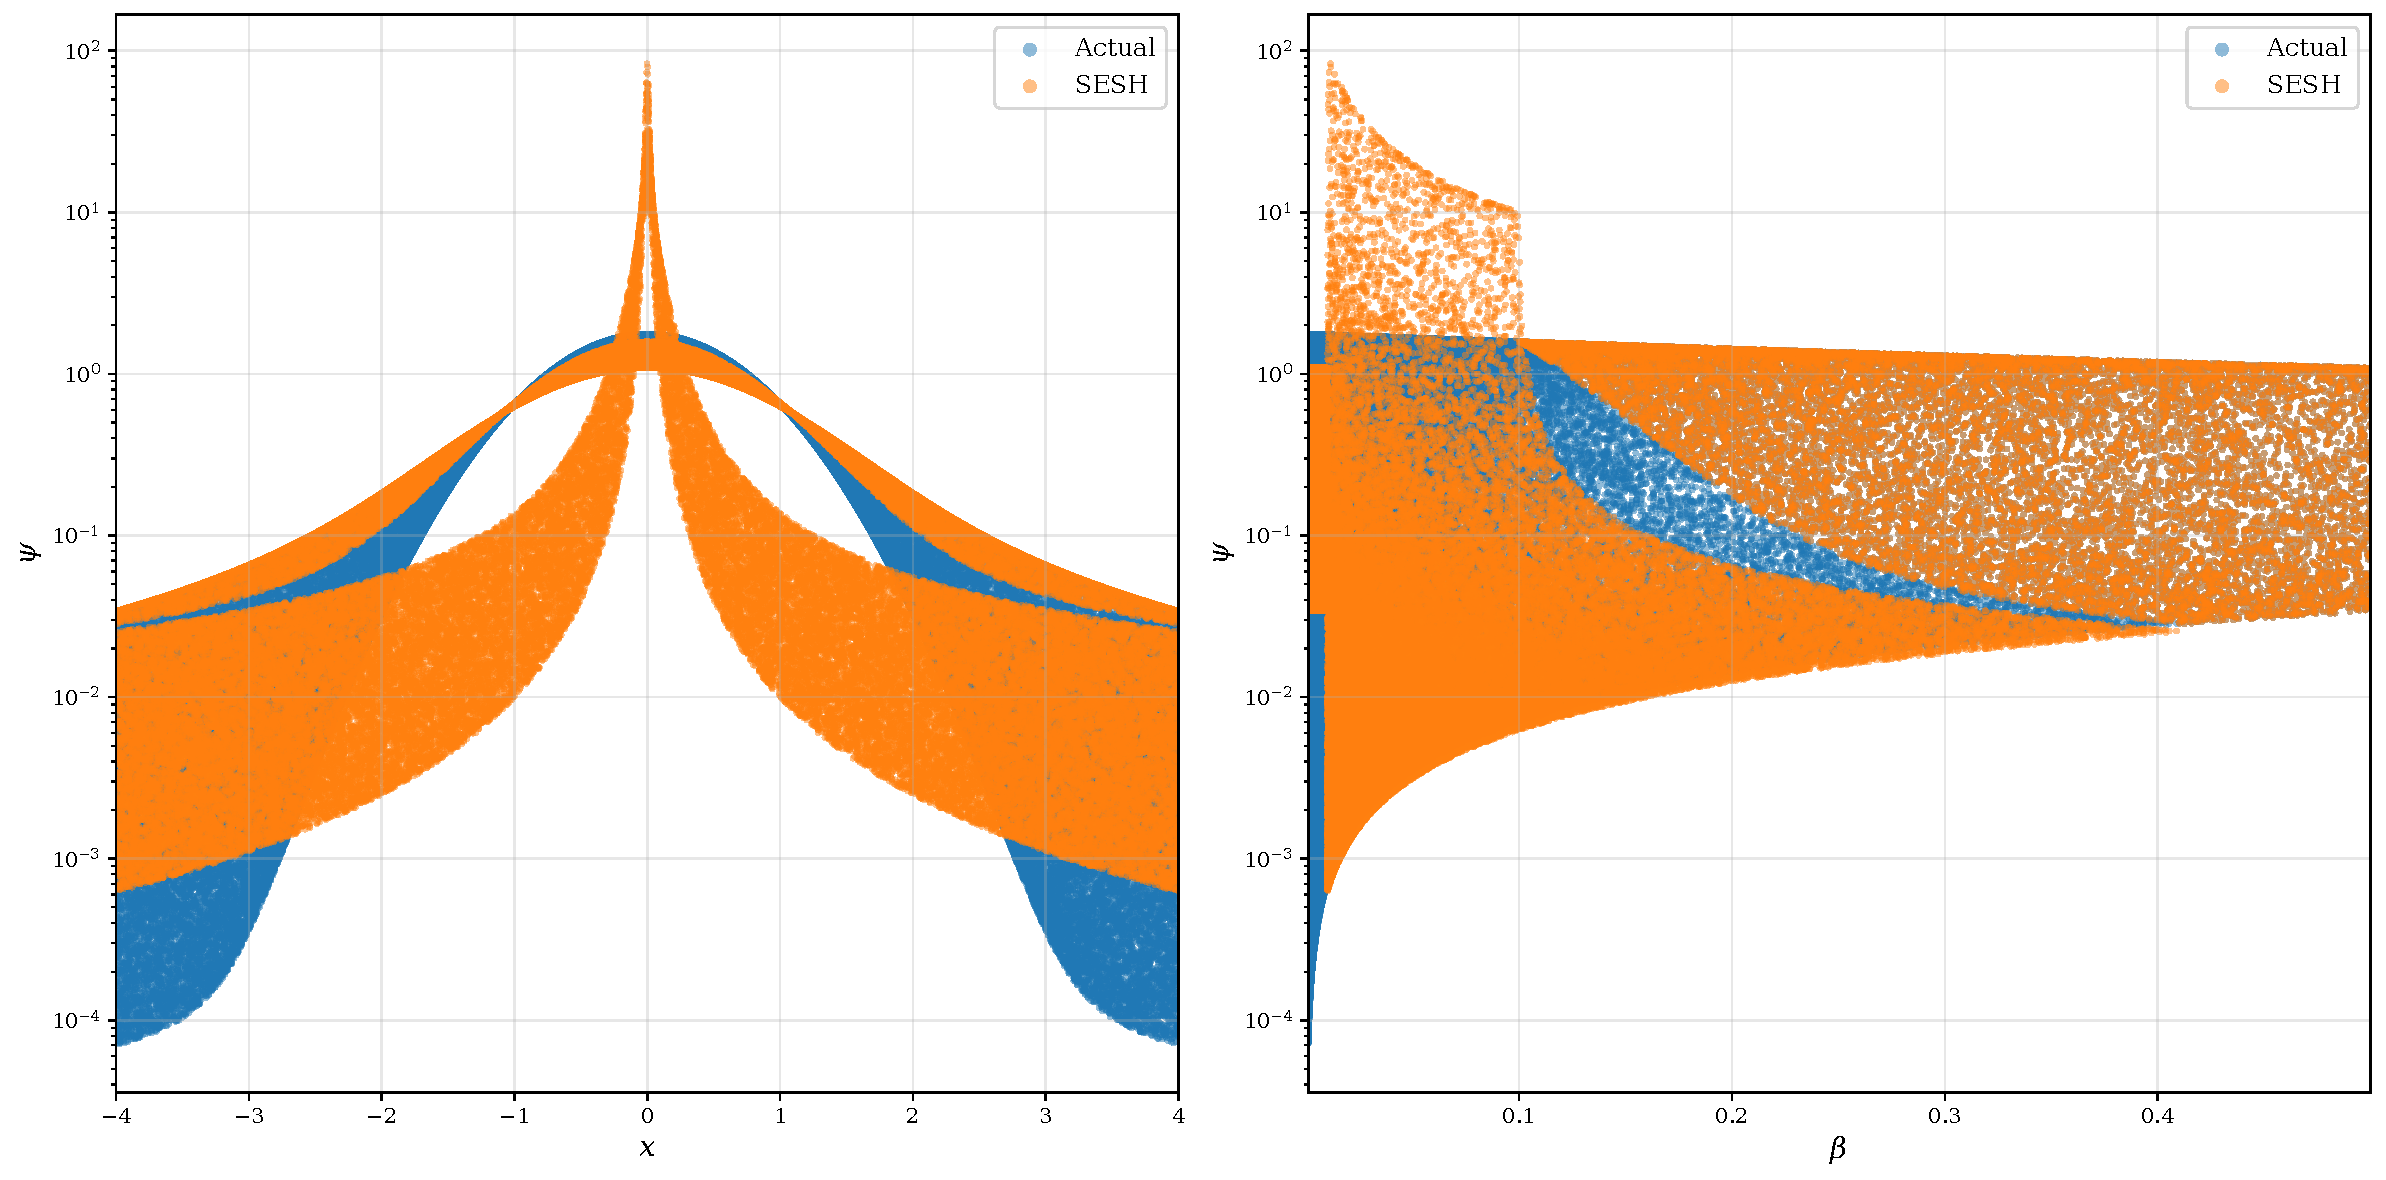
\includegraphics[width=0.99\linewidth]{Implementation/Figures/beta-error.pdf}
        \caption{Comparing results of SESH's Faddeeva function output with what the Faddeeva function actually calculates given the same inputs.}
        \label{fig:beta-error}
    \end{figure}
    
    One significant effect of this bug is due to the inverse relationship between $\beta$ and energy, shown in \autoref{eq:doppler-beta}. As the energy of the incident neutron increases, the probability of $\beta$ being sampled as less than 0.01 increases. Consequently, as energy increases, the probability of the 0 Kelvin cross section being returned also increased.

    The solution was to implement a newer computation of the Faddeeva function\cite{faddeeva}. This resolved the issues present in the original algorithm present in SESH, but also reduced error of the function at all values of $\beta$, shown in \autoref{fig:faddeeva-algorithm}.
    \begin{figure}[H]
        \centering
        \includegraphics[width=0.75\textwidth]{Implementation/Figures/DopplerBroadenedBeta.pdf}
        \caption{Faddeeva function error for old and new algorithms as a function of $\beta$.}
        \label{fig:faddeeva-algorithm}
    \end{figure}

\section{Cross-Section Validation}
    \label{sec:cross-section-validation}
    After implementing the cross-section generation module, it was necessary to validate its performance in calculating cross-section distributions. The goal was to ensure that the updated SESH could accurately reproduce cross-section distributions from the same set of resonance parameters.

    In order to perform this validation, the cross-section distribution of \textsuperscript{90}Zr at 200 keV was generated by SESH and FRENDY\cite{frendy}. Rather than using the \textsuperscript{90}Zr ENDF-8.1 evaluation for the FRENDY calculation, the ENDF file used by FRENDY was generated using SAMMY from the URR parameters described in \autoref{sec:urr-in-sammy}. This created a direct one-to-one comparison between models, such that the resonance parameters did not contribute to any discrepancy between the generated distributions. Further information regarding this step is discussed in greater detail in \autoref{chap:multiiso-transmission-correction}.

    \begin{figure}[h]
        \centering
        \includegraphics[width=0.95\linewidth]{Implementation//Figures/cross-section-validation.png}
        \caption{Validating SESH-calculated total cross-section generation with FRENDY calculation using identical resonance parameters}
        \label{fig:cross-section-validation}
    \end{figure}

    The comparison between the FRENDY-calculated and SESH-calculated total cross section distributions is given in \autoref{fig:cross-section-validation}. As the figure illustrates, there is very strong agreement throughout the entire distribution. This demonstrates that the underlying statistical behavior of the cross-sections are being modeled correctly.

    This agreement serves as validation of the new SESH implementation, confirming its physical accuracy by verifying two crucial aspects of its cross section generation:
    \begin{enumerate}
        \item \textbf{SESH and SAMMY are internally consistent.} This validation required calculating average channel-dependent parameters from $\ell$-dependent parameters. The identical distribution reflects that the channel-dependent parameters are consistent between code workflows.
        \item \textbf{SESH's Monte Carlo cross-section sampling is identical to current processing codes.} This validates the core functionality of SESH's cross-section sampling. Although the doppler broadening subroutines and weighted Wigner distribution are significantly different implementations from processing codes, SESH is able to return an identical total cross-section distribution.
    \end{enumerate}

